\def\CTeXPreproc{Created by ctex v0.2.9, don't edit!}
%\documentclass{beamer}
\documentclass[%handout,
xcolor=pdftex]{beamer}
\mode<presentation> {
  \usetheme{Warsaw}
  \setbeamercovered{transparent}
}
\let\Tiny=\tiny
\usetheme{Singapore}
\usecolortheme{dolphin}
\usepackage{amsmath}
\usepackage{textcomp}
\usepackage{amssymb}
\usepackage{amsthm}
\usepackage{graphicx}
\usepackage{color}
\usepackage{lipsum}
\usepackage{hyperref}
\usepackage{multirow}
\usepackage{bm}
%\setbeamertemplate{headline}{}
\setbeamertemplate{footline}[page number]
\newcommand\Fontvi{\fontsize{9pt}{8}\selectfont}
\newcommand\Fontvii{\fontsize{7pt}{8}\selectfont}
\newcommand{\backupbegin}{
   \newcounter{finalframe}
   \setcounter{finalframe}{\value{framenumber}}
}
\newcommand{\backupend}{
   \setcounter{framenumber}{\value{finalframe}}
}\newtheorem{proposition}{Proposition}
\title{Unit 13: ARMA Estimation}
\author[STAT 5170: Applied Time Series, Unit 13]{Jeffrey Woo}
\institute{Department of Statistics, University of Virginia}
\date{Spring 2020}

\AtBeginSubsection[] {
  \begin{frame}<beamer>{Outline}
    \tableofcontents[currentsection,currentsubsection]
  \end{frame}
}

\begin{document}


\frame{\titlepage}


\begin{frame}
\frametitle{Readings for Unit 13}

Textbook chapter 3.5 (pages 113 to 121).

\end{frame}



\begin{frame}
\frametitle{Last Unit}
\begin{enumerate}
\item ARMA forecasting.
\item Prediction error.
\item Prediction interval.
\end{enumerate}
\end{frame}

\begin{frame}
\frametitle{This Unit}
\begin{enumerate}
\item Method of Moments Estimation.
\item Maximum Likelihood Estimation.
\end{enumerate}
\end{frame}


\begin{frame}
\frametitle{Motivation}

In this unit, we explore a couple of ways to estimate the parameters for ARMA models: Method of Moments (MOM) estimation and Maximum Likelihood (ML) estimation.

\end{frame}

\section{Method of Moments Estimation}
\frame{\tableofcontents[currentsection]}

\begin{frame}
\frametitle{ARMA Estimation}

Let's assume that we have an ARMA model (which is of course causal and invertible)
$$
\phi(B)  X_t = \theta(B) w_t,
$$
where the white noise $w_t$ has variance $\sigma^2_w$,
$$
\phi(B) = 1-\phi_1 B - \cdots - \phi_p B^p \quad
\mbox{and} \quad
\theta(B) = 1+\theta_1 B + \cdots+\theta_q B^q.
$$
Given $n$ observations $x_1,x_2,\ldots,x_n$, we are interested
in estimating the parameters
$\phi_1,\ldots,\phi_p,\theta_1,\ldots,\theta_q$ and
$\sigma^2_w$. Initially we assume that the orders $p$ and $q$
are known.
\end{frame}

\begin{frame}
\frametitle{Method of Moments}

Let's start with the method of moments (MOM) estimation. The idea behind this is to equate population moments to sample moments and then solving for the parameters in terms of the sample moments.

\end{frame}

\begin{frame}
\frametitle{Method of Moments: Toy Example}



\end{frame}

%\begin{frame}
%\frametitle{Method of Moments: Example}

%\textbf{Question}: Consider $x_1, \cdots, x_n$ iid normal random variables with mean $\mu$ and variance $\sigma^2$. What are the MOM estimators of $\mu$ and $\sigma^2$?

%\vspace{50mm}
%\end{frame}


\begin{frame}
\frametitle{Yule-Walker Estimation for AR(p)}

The method of moments works well when estimating causal AR(p) models. We consider the causal AR($p$) model
\begin{eqnarray}\label{eq:1}
x_t=\phi_1 x_{t-1} + \cdots + \phi_p x_{t-p} + w_t.
\end{eqnarray}

Multiply both sides of (\ref{eq:1}) by $x_{t-h}$, and taking expectations, we obtain

\begin{eqnarray}\label{eq:2}
E (x_t x_{t-h})  = \hspace{50mm}
\end{eqnarray}


\end{frame}

\begin{frame}
\frametitle{Yule-Walker Estimation for AR(p)}

By definition of the autocovariance function,

\vspace{40mm}

We consider two cases.


\end{frame}

\begin{frame}
\frametitle{Yule-Walker Estimation for AR(p)}

\textbf{Case I}: $h \geq 1$. By causality, $x_{t-h}$ only depends on present and past white noise terms, $w_{t-h}, w_{t-h-1}, \cdots,$. Thus, $\mbox{E}(w_t x_{t-h}) = 0$. Then (\ref{eq:2}) becomes

\begin{equation} \label{eq:3}
\gamma(h) = \hspace{50mm}
\end{equation}

\end{frame}

\begin{frame}
\frametitle{Yule-Walker Estimation for AR(p)}

\textbf{Case II}: $h = 0$. Then

\begin{eqnarray} \label{eq:4}
\mbox{E}(w_t x_t) &=& \hspace{50mm} \nonumber \\
                  &=& \hspace{50mm} \nonumber \\
                  &=& \hspace{50mm}
\end{eqnarray}

due to causality $\mbox{E}(w_t x_{t-j}) = 0$ for $j \geq 1$.

\end{frame}

\begin{frame}
\frametitle{Yule-Walker Estimation for AR(p)}

\textbf{Case II (continued)}: Subbing (\ref{eq:4}) into (\ref{eq:2}), we obtain

\begin{eqnarray} \label{eq:5}
\gamma(0) &=& \hspace{50mm} \nonumber \\
          &=& \hspace{50mm}
\end{eqnarray}

\end{frame}

\begin{frame}
\frametitle{Yule-Walker Estimation for AR(p)}

We combine (\ref{eq:3}) and (\ref{eq:5}) to obtain the \textbf{Yule-Walker equations}

\begin{eqnarray*}
\gamma(h) &=&  \phi_1 \gamma(h-1) + \phi_2 \gamma(h-2) + \cdots + \phi_p \gamma(h-p),  \\
\sigma_{w}^2 &=& \gamma(0) - \phi_1 \gamma(1) - \phi_2 \gamma(2) - \cdots - \phi_p \gamma(p).
\end{eqnarray*}

\end{frame}

\begin{frame}
\frametitle{Yule-Walker Estimation for AR(p)}

In matrix notation, the Yule-Walker equations are

\begin{equation*}
\boldsymbol{\Gamma}_p \boldsymbol{\phi} = \boldsymbol{\gamma}_p
\end{equation*}

and

\begin{equation*}
\sigma_w^2 = \gamma(0) - \boldsymbol{\phi^{\prime}\gamma}_p,
\end{equation*}

where $\boldsymbol{\Gamma}_p = \{\gamma(k-j) \}_{j,k=1}^p$ is a $p \times p$ matrix, $\boldsymbol{\phi} = (\phi_1, \cdots, \phi_p)^{\prime}$ is a $p \times 1$ vector, and $\boldsymbol{\gamma}_p = (\gamma(1), \cdots, \gamma(p))^{\prime}$ is a $p \times 1$ vector.

\end{frame}

\begin{frame}
\frametitle{Yule-Walker Estimation for AR(p)}

Using method of moments, we replace $\gamma(h)$ with $\hat{\gamma(h)}$ and solve

\begin{equation*}
\boldsymbol{\hat{\phi}} = \hat{\boldsymbol{\Gamma}}_p^{-1} \hat{\boldsymbol{\gamma}}_p
\end{equation*}

and

\begin{equation*}
\hat{\sigma}_w^2 = \hat{\gamma}(0) - \hat{\boldsymbol{\gamma}}_p^{\prime} \hat{\boldsymbol{\Gamma}}_p^{-1} \hat{\boldsymbol{\gamma}}_p.
\end{equation*}

\end{frame}

\begin{frame}
\frametitle{Yule-Walker Estimation for AR(p)}

By factoring $\hat{\gamma}(0)$, the Yule-Walker estimates are

\begin{equation} \label{eq:s1}
\boldsymbol{\hat{\phi}} = \hat{\bm{R}}_p^{-1} \hat{\boldsymbol{\rho}}_p
\end{equation}

and

\begin{eqnarray} \label{eq:s2}
\hat{\sigma}_w^2 &=& \hat{\gamma}(0) \left[ 1 - \hat{\boldsymbol{\rho}}_p^{\prime} \hat{\bm{R}}_p^{-1} \hat{\boldsymbol{\rho}}_p \right] \nonumber \\
                 &=& \hat{\gamma}(0) \left[ 1 - \hat{\boldsymbol{\rho}}_p^{\prime} \boldsymbol{\hat{\phi}} \right],
\end{eqnarray}

where $\bm{\hat{R}}_p = \{\hat{\rho}(k-j) \}_{j,k=1}^p$ is a $p \times p$ matrix and $\boldsymbol{\hat{\rho}}_p = (\hat{\rho}(1), \cdots, \hat{\rho}(p))^{\prime}$ is a $p \times 1$ vector.

\end{frame}

\begin{frame}
\frametitle{Yule-Walker Estimation for AR(p)}

The asymptotic behavior of the Yule-Walker estimators for causal AR(p) processes is

\begin{equation} \label{eq:asymp}
\sqrt{n}\left(\hat{\bm{\phi}} - \bm{\phi}\right) \xrightarrow[]{d} N\left( \bm{0}, \sigma_w^2 \bm{\Gamma}_p^{-1} \right)
\end{equation}

and

\begin{equation*}
\hat{\sigma}_w^2 \xrightarrow[]{p} \sigma_w^2.
\end{equation*}

\end{frame}

\begin{frame}
\frametitle{Yule-Walker Estimation for AR(p)}

The variance-covariance matrix for $\hat{\bm{\phi}}$ is

\begin{eqnarray} \label{eq:varmatrix}
Var(\hat{\bm{\phi}}) &=& \frac{\sigma^2}{n} \bm{\Gamma}_p^{-1} \nonumber \\
                     &=& \frac{\sigma^2}{n\hat{\gamma}(0)}  \bm{R}_p^{-1}
\end{eqnarray}

\end{frame}


\begin{frame}[fragile]
\frametitle{Simulation Example}

Using the \verb=armasim()= function, I simulated $n=1000$ observations from the following AR(2) process

$$
x_t = 1.5 x_{t-1} - 0.75 x_{t-2} + w_t
$$

where $\sigma_w^2 = 1$. For the sample, $\hat{\gamma}(0) = 7.69697$, $\hat{\rho}(1)=0.8456375$, and $\hat{\rho}(2) = 0.5054795$.

\end{frame}

\begin{frame}
\frametitle{Simulation Example}



\end{frame}

\begin{frame}
\frametitle{Fish Population Example}

In Unit 11, we looked at the ACF and PACF of the time series from ``recruit.dat", which contains data on fish population in the central Pacific Ocean. The numbers represent the number of new fish for each month in the years 1950-1987. We decided that an AR(2) model is most appropriate.
\end{frame}

\begin{frame}
\frametitle{Fish Population Example}

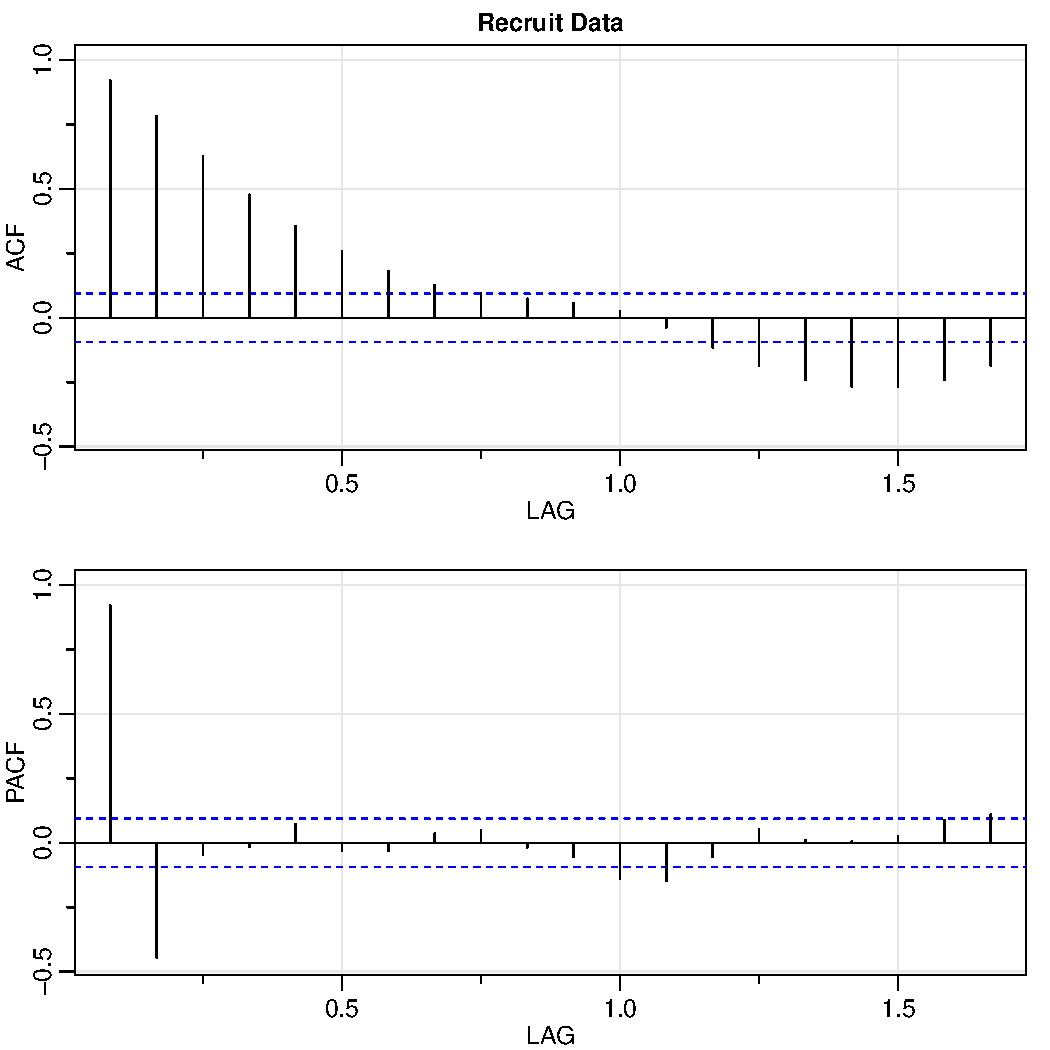
\includegraphics[width=100mm, height=80mm]{recruit.pdf}

\end{frame}

\begin{frame}[fragile]
\frametitle{Fish Population Example}

Let's check the results of fitting an AR(2) model using Yule-Walker estimation in R.

\begin{verbatim}
> rec.yw<-ar.yw(rec, order=2)
> rec.yw$x.mean
[1] 62.26278
> rec.yw$ar
[1]  1.3315874 -0.4445447
> sqrt(diag(rec.yw$asy.var.coef))
[1] 0.04222637 0.04222637
\end{verbatim}

\end{frame}

\begin{frame}
\frametitle{Fish Population Example}

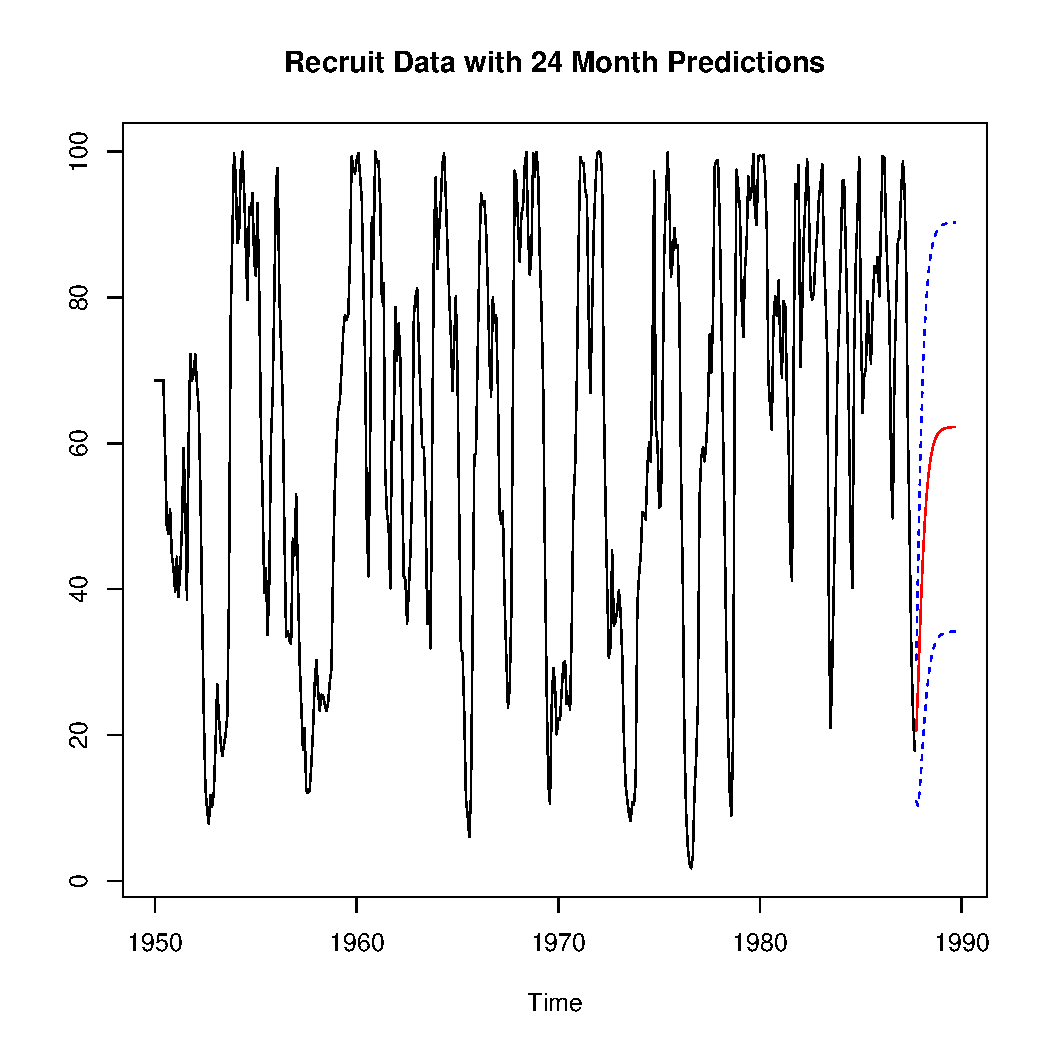
\includegraphics[width=100mm, height=80mm]{pred.pdf}

\end{frame}

\begin{frame}[fragile]
\frametitle{Fish Population Example}

\begin{verbatim}
rec.pred <- predict(rec.yw, n.ahead=24)
ts.plot(rec, rec.pred$pred, col=1:2, main="Recruit Data with 24 Month Predictions")
lines(rec.pred$pred - rec.pred$s, col=4, lty=2)
lines(rec.pred$pred + rec.pred$s, col=4, lty=2)
\end{verbatim}

\end{frame}

\begin{frame}
\frametitle{Method of Moments Estimation for MA(q)}

Consider an MA(1) process $x_t = w_t + \theta w_{t-1}$. We know that

$$
\rho(1) = -\frac{\theta}{1 + \theta^2}.
$$

Using method of moments, we equate $\hat{\rho}(1)$ to $\rho(1)$ and solve a quadratic equation in $\theta$.


\end{frame}

\begin{frame}
\frametitle{Method of Moments Estimation for MA(q)}

The invertible solution is

$$
\hat{\theta} = \frac{-1 + \sqrt{1 - 4 \hat{\rho}(1)^2}}{2 \hat{\rho}(1)}.
$$

If $\hat{\rho}(1)= \pm 0.5$, real solutions exist, $\mp 1$, neither is invertible. \\
If $\hat{\rho}(1)>0.5$, no real solutions exist, the method of moments fails to yield an estimator of $\theta$.

\end{frame}

\begin{frame}
\frametitle{Method of Moments Estimation for MA(q)}

For higher order MA(q) models, the method of moments quickly gets complicated. The equations are non-linear in $\theta_1, \cdots, \theta_q$, so numerical methods need to be used. \\
\vspace{5mm}
It turns out that for MA(q) models, method of moments produces poor estimates, in general.
\end{frame}

\section{Maximum Likelihood Estimation}
\frame{\tableofcontents[currentsection]}

\begin{frame}
\frametitle{Maximum Likelihood Estimation}

To illustrate the main concept with maximum likelihood estimation, we consider the AR(1) model with nonzero mean

\begin{eqnarray}\label{eq:ar1}
x_t=\mu+\phi(x_{t-1}-\mu)+w_t,
\end{eqnarray}

where $|\phi|<1$ and $w_t\sim iid $ N(0,$\sigma^2_w$).

\end{frame}

\begin{frame}
\frametitle{Maximum Likelihood Estimation}

We seek the likelihood
\begin{eqnarray}\label{eq:likelihood}
L(\mu,\phi,\sigma^2_w) = f_{\mu,\phi,\sigma^2_w}(x_1,x_2,\ldots,x_n).
\end{eqnarray}
Intuitively speaking, the likelihood function (\ref{eq:likelihood})
$L(\mu,\phi,\sigma^2_w)$ is formed from the joint probability distribution of the observed data $x_1,x_2,\ldots,x_n$ as a function of the parameters $\mu,\phi,\sigma^2_w$.

\end{frame}

\begin{frame}
\frametitle{Maximum Likelihood Estimation}

For given data, you can
think of the likelihood as a function of the parameters.
Since we've actually observed the data $x_1,x_2,\ldots,x_n$, we
can find parameters $(\mu,\phi,\sigma^2_w)$ to maximize the
likelihood $L(\mu,\phi,\sigma^2_w)$. This is the basic idea
behind maximum likelihood estimation.

\end{frame}


\begin{frame}
\frametitle{Likelihood Function}

Recall that, for two random variables $X$
and $Y$, the \underline{\hspace{20 mm}} $f_{X,Y}(x,y)$ of $(X,Y)$ can be
written as
\begin{eqnarray*}
f_{X,Y}(x,y)=f_X(x) f_{Y|X}(y|x),
\end{eqnarray*}
where $f_X(x)$ is the density function of $X$, and
$f_{Y|X}(y|x)$ is the conditional density function of $Y$ given
$X=x$. Similar idea also carries over to multivariate random
variables.

\end{frame}

\begin{frame}
\frametitle{Likelihood Function}

Since $w_t$ are iid normal random variables with variance
$\sigma^2_w$, in the case of (\ref{eq:ar1}), we have
\begin{eqnarray*}
x_2|x_1 =\mu+\phi(x_1-\mu) + w_2|x_1 \sim N(\mu+\phi(x_1-\mu),\sigma^2_w)
\end{eqnarray*}
and
\begin{eqnarray*}
 f_{x_2|x_1}(x_2|x_1) = \frac{1}{\sqrt{2\pi \sigma_w^2}}
\exp \Big \{-\frac{[x_2-\mu-\phi(x_1-\mu)]^2}{2\sigma^2 _w} \Big \}.
\end{eqnarray*}


\end{frame}

\begin{frame}
\frametitle{Likelihood Function}

Similarly,
\begin{eqnarray*}
f_{x_t|x_{t-1}}(x_t|x_{t-1}) = \frac{1}{\sqrt{2\pi \sigma_w^2}}
\exp \Big \{-\frac{[x_t-\mu-\phi(x_{t-1}-\mu)]^2}{2\sigma^2 _w} \Big \}.
\end{eqnarray*}

\end{frame}

\begin{frame}
\frametitle{Likelihood Function}

We have
\begin{eqnarray}\label{eq:cle}
L(\mu,\phi,\sigma^2_w) &=& f_{x_1}(x_1) \times f_{x_2|x_1}(x_2|x_1) \times \cdots \times f_{x_n|x_{n-1}}(x_n|x_{n-1}) \cr
&=& f_{x_1}(x_1) (2\pi \sigma^2_w)^{-(n-1)/2} \exp \Big \{ -\frac{S(\mu,\phi)}{2\sigma^2_w} \Big \},
\end{eqnarray}
where
\begin{eqnarray*}
S(\mu,\phi) = \sum^n_{t=2} [x_t-\mu-\phi(x_{t-1}-\mu)]^2.
\end{eqnarray*}

\end{frame}


\begin{frame}
\frametitle{Likelihood Function}

Note that for the AR(1) model (\ref{eq:ar1}), we have the
causal representation $x_1=\mu+\sum^\infty_{j=0} \phi^j
w_{1-j}$. Since $w_t$ are iid normal, $x_1$ is a normal with
mean $\mu$ and variance $\sigma^2_w/(1-\phi^2)$, and
\begin{eqnarray*}
f_{x_1}(x_1)=\frac{1}{\sqrt{2\pi \sigma^2_w/(1-\phi^2)}}
\exp \Big \{- \frac{(x_1-\mu)^2}{2\sigma^2_w/(1-\phi^2)} \Big \}
\end{eqnarray*}

\end{frame}

\begin{frame}
\frametitle{Likelihood Function}

Thus, for given data $x_1,x_2,\ldots,x_n$, we can find
$(\mu,\phi,\sigma^2_w)$ to maximize the likelihood
$L(\mu,\phi,\sigma^2_w)$ in (\ref{eq:cle}). It is worth
pointing out that it is more common to consider the log-likelihood
\begin{eqnarray*}
\ell(\mu,\phi,\sigma^2) = \log L(\mu,\phi,\sigma^2).
\end{eqnarray*}

Maximizing log-likelihoods may not always have a closed-form solution. \underline{\hspace{30 mm}} (e.g.: Newton-Raphson, Fisher scoring) needed.

\end{frame}

\begin{frame}
\frametitle{Properties of Maximum Likelihood Estimators}

Maximum likelihood estimators are approximately unbiased and normally distributed, for large $n$.
\end{frame}

\section{Comparison of MOM and MLE}
\frame{\tableofcontents[currentsection]}


\begin{frame}
\frametitle{Properties of Method of Moment Estimators}

Advantages:

\begin{itemize}
\item Efficient (\underline{\hspace{35 mm}}) for AR(p) models.
\item Nice closed-form solutions for AR(p) models.
\end{itemize}

Disadvantages:

\begin{itemize}
\item Poor efficiency for MA(q) models.
\end{itemize}

\end{frame}

\begin{frame}
\frametitle{Properties of Maximum Likelihood Estimators}

Advantages:

\begin{itemize}
\item Efficient.
\item Even if $x_t$ is not Gaussian, the asymptotic distribution of the MLE is the same when $x_t$ is Gaussian.
\end{itemize}

Disadvantages:

\begin{itemize}
\item Difficult optimization problem.
\item Need to choose a good starting point.
\end{itemize}

\end{frame}

\end{document} 